%%%------Preambulo------%%%

%Tipo de documento:
\documentclass{book}

%Este paquete es utilizado para personalizar elementos por idioma:
\usepackage[spanish,mexico]{babel}

%Este paquete es utilizado para la codificac\'on de entrada:
\usepackage[utf8]{inputenc}

\usepackage{amssymb}

\usepackage{graphicx}

\usepackage{verbatim}

%Otras declaracines:
%Cada vez que se compila la fecha se actualiza

\begin{document}

\chapter{Conceptos b\'asicos}
Computadora : M\'aquina electronica de c\'alculo, compuesta por circuitos l\'ogicos que generan conexiones.\\

Componentes de circuitos lógicos 
\begin{itemize}
\item Amplificador operacional:
\item Biestable:
\item PDL:
\item Diac:
\item Diodo:
\item FGPA: 
\item Memoria:
\item Microprocesador:
\item Pila:
\item Tiristor:
\item Puerta l\'ogica:
\item Transistor:
\item Triac: 
\end{itemize}

%----Faltan imagenes de los elementos----%

%----Tabla de almacenamiento de datos-----%

\section{Componentes electr\'onicos}
%---Definir un poco---%
\subsection{Componentes electr\'onicos pasivos}
Los componentes electr\'onicos pasivos son elementos que act\'uan como cargas de manera que no generan ni amplifican la se\~nal. No necesitan polarizaci\'on.
\begin{itemize}
\item Resistores: Es la mayor o menor oposici\'on que presenta el elemento del circuito al paso de la corriente el\'ectrica.
\item Condensadores: Componente capaz de almacenar temporalmente cargas electr\'onicas
\item Inductores (bobinas): Son elementos lineales y pasivos que pueden almacenar y liberar energ\'ia bas\'andose en fen\'omenos relacionados con campos magn\'eticos.
\end{itemize}

\subsection{Componentes electr\'onicos activos}
Los componentes electr\'onicos activos son capaces de generar, modificar y amplificar el valor de una se\~nal el\'ectrica.

\begin{itemize}
\item Diodos: Son aquellos materiales que a temperatura ambiente tienen una resistencia que se halla comprendida entre la de los metales y los aislantes.
\item Transistores: Dispositivo que regula el flujo de corriente o de tension actuando como un interruptor o amplificador para se\~nales electr\'onicas.
\item Circuitos integrados: Es una pastilla o chip muy delgado en el que se encuentran una cantidad enorme de dispositivos microelectr\'onicos.
\end{itemize}

\section{Representaci\'on de punto flotante}


%----Ilustración de cadena-----%
\begin{figure}[h]
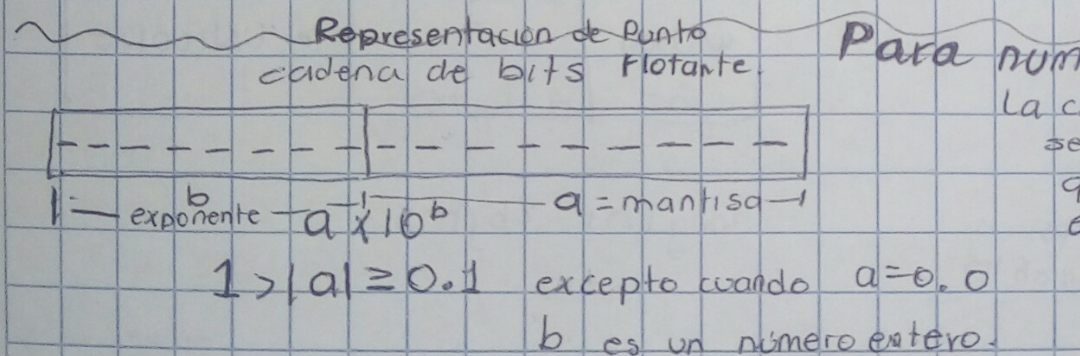
\includegraphics[scale=.16]{cadena-de-bits}
\centering
\caption{Cadena de bits.}
\end{figure}

\begin{center}
$a \times 10^b$\\
$0.1 \leq |a| < 1$\\
exceptuando cuando: $a=0.0b$ \\ 
\bigskip
\begin{tabular}{| c | c |}
\hline
Tipo de datos & Espacio de almacenamiento\\
\hline 
float& 4 bytes\\
double & 8 bytes\\
long double & 16 bytes\\
\hline
\end{tabular}
\end{center}

\section{Tipos de error}

\subsection{Error de corte}
Depende de la m\'aquina, es un error num\'erico,. P\'erdida de cifras significativas cuando sumamos o restamos cantidades con diferente orden de magnitud.\\
%poner ejemplo%

Epsil\'on de la m\'aquina (EPS): Es el n\'umero m\'as pequeño tal que $(1+EPS)\textgreater1$ para la m\'aquina que realiza la suma.
El siguiente c\'odigo permite conocer el epsil\'on de tu computadora.
\medskip
\begin{verbatim}
double EPS=1.0;
int k=0;
while((EPS+1.0)>1.0){
      EPS/=2.0;
      K++
      }
EPS*=2.0;
K--;
printf("Epsilon de la maquina = %f", EPS);
printf("\n Equivalente a 2^ %d", k);
\end{verbatim}

\subsection{Error de redondeo} 
P\'erdida de cifras decimales a medida que se aumenta el exponente.

%----Ilustración de recta-----%
\begin{figure}[h]
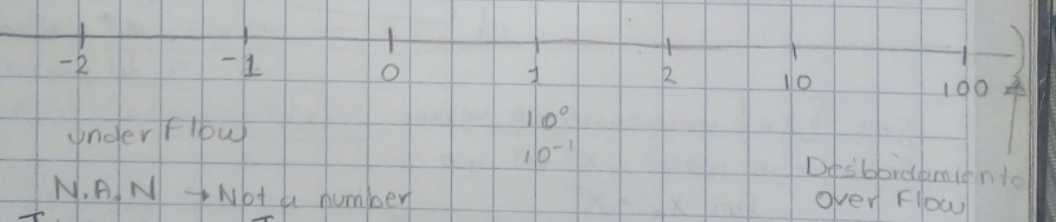
\includegraphics[scale=.16]{recta-error-redondeo}
\centering
\caption{Recta que ejemplifica el error de redondeo.}
\end{figure}

\subsection{Error de truncamiento}
Son aquellos que resultan al usar una aproximaci\'on en lugar de un procedimiento matem\'atico exacto.\\
Ejemplo:\\
Teorema de Taylor: Si $f(x)$ es una funci\'on suave en un intervalo abierto $(a,b)$ que contiene a $c$, para un n\'umero $c+h$ contenido en $(a,b)$ \\
$f(c+h)=f(c)+f'(c)h+f''(c)\frac{h^2}{2!}+f'''(c)\frac{h^3}{3!}+...+f^n(c)\frac{h^n}{n!}$ \\
El hecho de perder cifras debido a limitar el resultado a ciertas decimales es a lo que llamamos error de truncamiento.\\

\subsection{Complejidad algor\'itmica y costo computacional}
%---Diagramas---%

\begin{center}
\textbf{Tiempo de tendencia a funciones}\\
\begin{tabular}{| c | c |}
\hline
$\log(n)$ & \\
$n$ & Tiempos lineales \\ 
$n\log(n)$ & \\
\hline
$n^2$ & \\
$n^3$ & Tiempos polin\'omicos \\ 
$n^4$ & \\
\hline
$2^n$ & NP-Duro \\
$n!$ & NP-Cmpleto\\
\hline
\end{tabular}
\end{center}
%-Ilustracion de grafica log-%
\begin{figure}[h]
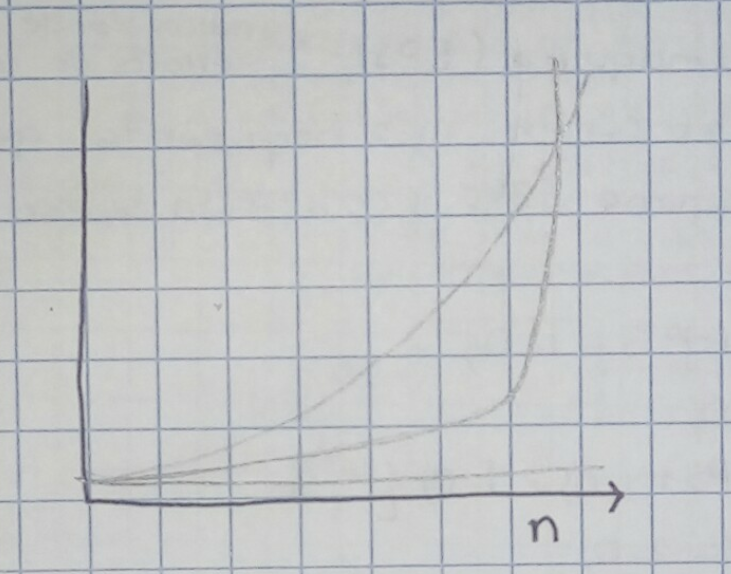
\includegraphics[scale=.16]{grafica-log}
\centering
\caption{Gr\'afica que estaba junto a lo de "Tiempo de tendencia de funciones".}
\end{figure}

\subsection{Convergencia} 
Un ciclo de c\'alculo se traduce a una iteraci\'on. \\

%--Ilustración de iteración--%
\begin{figure}[h]
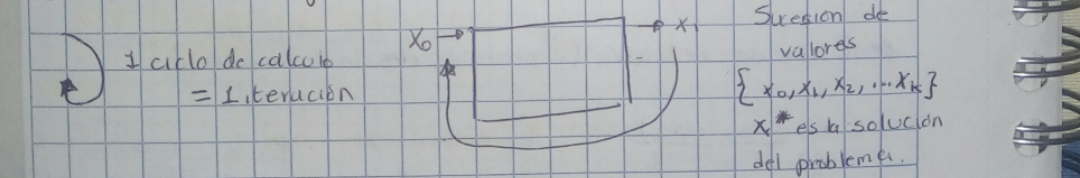
\includegraphics[scale=.16]{iteracion}
\centering
\caption{Iteraci\'on.}
\end{figure}

Sea $x_k$ una sucesi\'on de valores. Si existe un n\'umero $x^*$ tal que $$\lim\limits_{k\to\infty}x_k=x^*$$ \\
La sucesi\'on converge a $x^*$, si eso no ocurre, entonces la sucesi\'on diverge.
\\
\textbf{Velocidad de convergencia}\\ 
%--Ilustración de iteración--%
\begin{figure}[h]
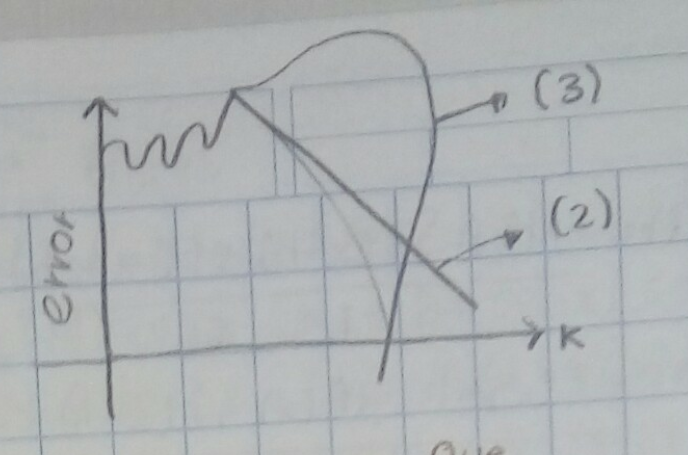
\includegraphics[scale=.16]{grafica-junto-vel-conv}
\centering
\caption{No estoy muy segura de la raz\'on de ser de la gr\'afica, pero estaba a un lado.}
\end{figure}

${x_k}$ converge a $x^*$ \\
\begin{enumerate}
\item Si existe un $k\geq 1$ a partir del cual se observa que $|x_{k+1}-x^*|\leq C|x_k-x^*|$ donde $C$ es constante entre $(0,1)$ se tiene velocidad de convergencia lineal.
\item Igual que el anterior pero $|x_{k+1}-x^*|\leq c_k|x_k-x^*|$ con $c_k\exists(0,1)$ y $C_k\to0$ cuando $k\to\infty$, se tiene  velocidad de convergencia lineal.
\item A partir de la iteraci\'on $k$ se observa que $|x_{k+1}-x^*|\leq C{|x_k-x^*|}^P$ donde $C$y $P$ son constantes $C\in(0,1)$ y $P\geq2$, se tiene convergencia de orden $P$.
\end{enumerate}


\chapter{Derivadas n\'umericas}
%-----Concepto básico de derivada númerica y utilidad------%
\begin{center}
\begin{eqnarray}
\nonumber
\frac{d(f(x))}{dx}=\lim\limits_{\Delta x\to0}\frac{f(x+\Delta x)-f(x)}{\Delta x} \qquad\nonumber h\geq\sqrt{EPS}
\end{eqnarray}
\end{center}
\begin{tabular}{ l }
 Derivada n\'umerica hacia adelante \\
$f'(x)\thickapprox \frac{f(x+h)-f(x)}{h}$ \\
\\
 Derivada n\'umerica hacia atr\'as \\
$f'(x)\thickapprox \frac{f(x)-f(x-h)}{h}$ \\
\\
 Derivada n\'umerica al centro \\
$f'(x)\thickapprox \frac{f(x+h)-f(x-h)}{2h}$ \\
\\
\end{tabular}
\\
Para el c\'alulo de derivadas n\'umericas se parte del analis\'is de una segunda deribada hacia adelante.\\
\begin{displaymath}
f''(x)=\frac{f'(x+h)-f'(x)}{h}=\frac{\frac{f(x+2h)-f(x+h)}{h}-\frac{f(x+h)-f(x)}{h}}{h}
\end{displaymath} 
\\De la cual obtenemos la ecuaci\'on para calcular $f''$ hacia adelante\\ \\
\begin{tabular}{  l  }
$f''(x)=\frac{f(x+2h)-2f(x+h)+f(x)}{h^2}$ \\
Segunda derivada n\'umerica hacia adelante \\
\\
$f''(x)=\frac{f(x)-2f(x-h)+f(x-2h)}{h^2}$ \\
Segunda derivada n\'umerica hacia atr\'as \\
\\
$f''(x)=\frac{f(x+h)-2f(x)+f(x-h)}{h^2}$ \\
Segunda derivada n\'umerica al centro \\
\\
\end{tabular}
\\
Para obtener un buen resultado en en el c\'alculo de segundas derivadas num\'ericas es necesario que $h\geq\sqrt[3]{EPS}$ \\ \\ \\
Ejemplo\\ \\
C\'alcular la $1^{ra}$ y $2^{da}$ derivada en $x=0.78$ de la funci\'on $3x^2\sin^2x$\\ \\
Anal\'iticamente \\
\begin{displaymath}
u=3x^2\quad v=\sin^2x
\end{displaymath}

\chapter{Soluci\'on de ecuaciones algebraicas}


Hay ocaciones en las que ecuaciones algebraicas tienen una dificil soluci\'on anal\'itica y en esas cituaciones recurrimos a los m\'etodos num\'ericos que ser\'an descritos en este cap\'itulo, hablaremos de m\'etodos tanto abiertos como cerrados, ventajas y desventajas de los mismos. 

\section{M\'etodos cerrados}
Tambi\'en llamados metodos de encierro, se basan en limitar con un intervaloque se va recortando hasta que se acerca a la soluci\'on.

\subsection{Bisecci\'on}
Es un algoritmo de b\'usqueda de ra\'ices que trabaja dividiendo el intervalo a la mitad y seccionando el subintervalo que tiene la ra\'iz, y es posible describirlo en los siguientes pasos.\\
\begin{enumerate}
\item Se eligen los valores limitantes $a$,  $b$ tales que \\$f(a)f(b)\textless0$.
\item aproximamos la soluci\'on con la formula del punto medio\\$c=\frac{a+b}{2}$
\end{enumerate}
%-----Gráfica del método de bisección-----%
%------Algoritmo de bisección-------%
\subsection{M\'etodo de falsa posici\'on o regula fals}
Para localizar el punto $c$, se busca la ecuaci\'on de una recta que pasa por los dos puntos de la funci''on lo que se obtiene es una ra\'iz falsa con una recta el presedimiento se muestra descrito en el siguiente algoritmo.
%----Gráfica del metodo regula fals----%
%-------Algoritmo de falsa posicón-------% 

\section{M\'etodos abiertos}
Son m\'etodos en los que solo necesitamos un valor inicial al que llamamos $x_0$ y son capaces de encontrar ra\'ices tangentes al eje x.

\subsection{M\'etodo de Newton-Raphson}
Consiste en sacas la ecuaci\'on de las tangentes de la funci\'on.
\begin{gather}
y-f(x_o)=f'(x_o)(x-x_0) \\
x_1=x_o-\frac{f(x_1)}{f'(x_1)} \\
x_2=x_1-\frac{f(x_1)}{f'(x_1)} \\
\boxed{x_{k+1}=x_k-\frac{f(x_k)}{f'(x_k)}}
\end{gather}
%Gráfica del método de Newton Raphson%
\subsubsection*{C\'alculo de error}

\subsection{M\'etodo Secante}
Se trata de un m\'etodo donde se traza una recta secante entro los \'ultimos 2 puntos. Se utilizan derivadas centrales para m\'as precisi\'on y el costo computacional sea menor.
\begin{gather}
\nonumber(x_k,f(x_k+1)) \qquad (x_k,f(x_k))\\
y-f(x_k)=\frac{f(x_k)-f(x_{k-1})}{x_k-x_{k-1}}\\
\boxed{x_{k+1}=x_k-\frac{f(x_k)}{\frac{f(x_k)-f(x_{k-1})}{x_k-x_{k-1}}}}
\end{gather}
%----Grafica de Método de secante y código----%
\section*{Backtracking}
Es un m\'etodo de b\'usqueda de soluciones exhaustiva sobre grafos dirigidos a ciclos, el cual se acelera mediante poda de ramas poco prometedoras. Es decir se trata de buscar estados soluci\'on del problema. \\
\\
Las condiciones de partida son:
\begin{enumerate}
\item Alcanza la soluci\'on
\item Se alcanzan todos los estados sde soluci\'on
\end{enumerate}


\section*{Resumen del c\'apitulo}
Los m\'etodos aqu\'i mostrados son utilizadon para encontrar ra\'ices de funciones y todos llevan al mismo resultado, la gran diferencia esta en el tiempo de computo utilizado para el resultado y la presici\'on de este.\\
\\
\subsection*{Velocidad de convergencia}
La velocida de convergencia que hace referencia al timepo que tarda el ordenador en arrojar un resultado, se muestra en seguida para m\'etodos cerrados y abiertos 
\\
\begin{center}
\begin{tabular}{	c		c	}
M\'etodos & Velocidad de convergencia \\
Bisecci\'on & Lineal [Lento] \\
Falsa posici\'on & Lineal y super lineal \\
Newton-Raphson & Cuadr\'atica [R\'apido] \\
Secante & Cuadr\'atica [R\'apido] \\
\end{tabular}
\end{center}

\subsection*{Iteraciones con y sin backtraking en metodos abiertos}
Si el algoritmo converge en $k$ iteraciones :
\begin{center}
\begin{tabular}{	c		c	}
Newton-Raphson & $2k_1$ \\
Secante & $k_2+1$ \\
Newton-Raphson con B. & $2k_3+Nb_1$ \\
Secante con B. & $k_4+1+Nb_2$
\end{tabular}
\end{center}

\chapter{Soluci\'on de sistemas de ecuaciones}
El objetivo de estos m\'etodos es encontrar un vector soluci\'on para una matriz dada partiendo de la ecuaci\'on $Ax=b$. En este cap\'itulo se describir\'an m\'etodos directos y m\'etodos iterativos. Y lo primero es recordar algunas operaciones y propiedades b\'asicas de las matrices vistas en \'Algebra lineal. 

\section{Operaciones algebr\'aicas con matrices}
\subsection{Suma de matrices}
Es posible sumar dos matrces siempre y cuado sean del mismo tamaño haciendo una adici\'on de sus elementos correspondientes.\\
S\'i $A=[a_{ij}]$ y $B=[b_{ij}]$ son matrices del mismo tamaño $m \times n$, entonces su suma es la matriz de tamaño $m \times $. \\
\begin{center}
$A+B=[a_{ij}+b_{ij}]$
\end{center}
\subsection{Multiplicaci\'on por un escalar}
Si $A=[a_{ij}$es una matriz de tamaño $m \times n$ y $c$ es un escalar, entonces el multiplo escalar de $A$ por $c$ es la matriz de tamaño $m \times n$ dada por:
\begin{center}
$cA=[ca_{ij}]$
\end{center}  
\subsection{Multiplicaci\'on de matrices}
Si $A=[a_{ij}]$ es una matriz de $m \times n$ y $B=[b_{ij}]$ es una matriz de $m \times p$, entonces el producto $AB$ es una matriz de $m \times p$
\begin{center}
Sea $A=\begin{bmatrix}
a_{11} & a_{12}\\
a_{21} & a_{22}\\
a_{31} & a_{32}
\end{bmatrix}$ y $B=\begin{bmatrix}
b_{11} & b_{12}\\
b_{21} & b_{22}
\end{bmatrix}$ entonces \bigskip \bigskip .
$AB=\begin{bmatrix}
a_{11} & a_{12}\\
a_{21} & a_{22}\\
a_{31} & a_{32}
\end{bmatrix}
\begin{bmatrix}
b_{11} & b_{12}\\
b_{21} & b_{22}
\end{bmatrix}=
\begin{bmatrix}
a_{11}b_{11}+a_{12}b_{21} & a_{11}b_{12}+a_{12}b_{22}\\
a_{21}b_{11}+a_{22}b_{21} & a_{21}b_{12}+a_{22}b_{22}\\
a_{31}b_{11}+a_{32}b_{21} & a_{31}b_{12}+a_{32}b_{22}
\end{bmatrix}$
\end{center}
\subsection{Transpuesta de una matriz}
La transpuesta de una matriz se forma al escribir sus columnas como renglones. Por ejemplo, si $A$ es la matriz de $m \times n$ dada por:
\begin{center}
$A=\begin{bmatrix}a_{11} & a_{12} & a_{13} & \cdots &a_{1n} \\ a_{21} & a_{22} & a_{23} & \cdots & a_{2n}\\ a_{31} & a_{32} & a_{33} & \cdots & a_{3n} \\
\vdots & \vdots & \vdots & \ddots & \vdots\\
a_{m1} & a_{m2} & a_{m3} & \cdots & a_{mn}
\end{bmatrix}$; \bigskip 
 $A^T=\begin{bmatrix}a_{11} & a_{21} & a_{31} & \cdots &a_{m1} \\ a_{12} & a_{22} & a_{32} & \cdots & a_{m2}\\ a_{13} & a_{23} & a_{33} & \cdots & a_{m3} \\
\vdots & \vdots & \vdots & \ddots & \vdots\\
a_{1n} & a_{2n} & a_{3n} & \cdots & a_{mn}
\end{bmatrix}$
\end{center}
\subsection{Matriz sim\'etrica}
Una m\'atriz $A$ es simetrica si $A=A^T$. Partiendo de esta definici\'on, es evidente que una matriz sim\'etrica debe ser cuadrada. Existen cuatro importantes propiedades de matrices simetricas las cuales son:
\begin{enumerate}
\item $(A^T)^T=A$
\item $(A+B)^T=A^T+B^T$
\item $(cA)^T=c(A)^T$
\item $(AB)^T=B^TA^T$
\end{enumerate}
\subsection{Inversa de una matriz}
Una matriz $A$ de $n \times n$ es invertible (o no singular) si existe una matriz $B$ de $n \times n$ tal que $AB=BA=I$, donde $I$ es la matriz identidad de orden n. La matriz $B$ se denomino inversa (multiplicativa) de $A$.\\
Las matrices no cuadradas no tienen inversa.\\
Si A es una matriz invertible, entonces su inversa es \'unica y se denota por $A^{-1}$.
\begin{center}
$AX=I \quad$ Donde $X$ es la matriz inversa.
\end{center}
\subsection{Determinante de una matriz}
El determinante de una matriz est\'a dado por
\begin{center}
$A=\begin{bmatrix}a_{11} & a_{12}\\ a_{21} & a_{22} \end{bmatrix} ; \quad det(A)=|A|=a_{11}a_{22}-a_{21}a_{12}$
\end{center}
El determinante es la diferencia de los products de dos diagonales de la matriz. Si $A$ es una matriz triangular de orden $n$, su determinante es el producto de los elementos en la diagonal principal, $det(A)=|A|=a_{11}a_{22}a_{33}\cdots a_{nm}$
\section{Descomposici\'on matricial}
La descomposici\'on matricial es una forma de factorizaci\'on de matrices en distintas formas para diferentes propositos y resultados. Las principales descomposiciones son descritas a continuaci\'on 
\subsection{Matriz triangular inferior}
Una matriz con una trangulaci\'on inferior la podemos obtener de como producto de la siguiente formula.
\begin{displaymath}
\nonumber x_i=\frac{b_i-\sum_{k=1}^{i-1}a_{ik}x_k}{a_{ii}} 
\end{displaymath}
\begin{center}
$\begin{bmatrix} a_{11} & 0 & 0 & 0 \\
				 a_{21} & a_{22} & 0 & 0 \\
				 a_{31} & a_{32} & a_{33} & 0 \\
				 a_{41} & a_{42} & a_{43} & a_{44}
\end{bmatrix}\begin{bmatrix} x_1 \\
							 x_2 \\
							 x_3 \\
							 x_4 \\
\end{bmatrix} = \begin{bmatrix} b_1 \\
							   b_2 \\
							   b_3 \\
							   b_4 
\end{bmatrix}$
\end{center}
\subsection{Matriz triangular superior}
El contrario de la matris triangular inferior, esta la matriz triangular superior.
\begin{displaymath}
\nonumber x_i=\frac{b_i-\sum_{k=i+1}^{n}a_{ik}x_k}{a_{ii}} 
\end{displaymath}
\begin{center}
$\begin{bmatrix} a_{11} & a_{12} & a_{13} & a_{14} \\
				 0 & a_{22} & a_{23} & a_{24} \\
				 0 & 0 & a_{33} & a_{34} \\
				 0 & 0 & 0 & a_{44}
\end{bmatrix}\begin{bmatrix} x_1 \\
							 x_2 \\
							 x_3 \\
							 x_4 \\
\end{bmatrix} = \begin{bmatrix} b_1 \\
							   b_2 \\
							   b_3 \\
							   b_4 
\end{bmatrix}$
\end{center}
\section{M\'etodos directos}
Los m\'etodos directos se encargan de transforman el sistema original en otro equivalente y f\'acil de reolver.
\subsection{Eliminaci\'on Gaussiana}
\subsection{Factorizaci\'on LU}
\begin{center} $LU \qquad A=LU$ \end{center}
\begin{center} $\begin{bmatrix}
			      a_{11} & a_{12} & a_{13} & a_{14}\\
			      a_{21} & a_{22} & a_{23} & a_{24}\\
			      a_{31} & a_{32} & a_{33} & a_{34}\\
			      a_{41} & a_{42} & a_{43} & a_{44}
			      
\end{bmatrix}= \begin{bmatrix}
			       1 & 0 & 0 & 0\\
			      l_{21} & 1 & 0 & 0\\
			      l_{31} & l_{32} & 1 & 0\\
			      l_{41} & l_{42} & l_{43} & 1
\end{bmatrix} \begin{bmatrix}
                  u_{11} & u_{12} & u_{13} & u_{14}\\
			      0 & u_{22} & u_{23} & u_{24}\\
			      0 & 0 & u_{33} & u_{34}\\
			      0 & 0 & 0 & u_{44}
\end{bmatrix} $
\end{center}
\subsubsection{Doolittle}
La condici\'on para esta factorizaci\'on es:
\begin{center}
$l_{ii}=1$
\end{center}
\begin{displaymath}
L_{ij}=\frac{a_{ij}-\sum_{k=1}^{j-1}l_{ik}u_{kj}}{u_{jj}} \qquad U_{ij}=a_{ij}-\sum_{k=1}^{i-1}l_{ik}u_{kj}
\end{displaymath}
\subsubsection{Crout}
Mientras que para la factorizaci\'on de Crout es:
\begin{center}
$u_{ii}=1$
\end{center} 
\begin{displaymath}
L_{ij}=a_{ij}-\sum_{k=1}^{j-1}L_{ik}U_{kj} \qquad U_{ij}=\frac{a_{ij}-\sum_{k=1}^{j-1}L_{ik}U_{kj}}{L_{ii}}
\end{displaymath}
\subsubsection{Resultados}
\begin{multicols}{2}
$a_{11}=u_{11}$ \\
$a_{12}=u_{12}$ \\
$a_{13}=u_{13}$ \\
$a_{14}=u_{14}$ \\
$a_{21}=l_{21}u_{11}$ \\
$l_{21}=\frac{a_{21}}{u_{11}}$ \\
$u_{22}=l_{21}u_{12}+u_{22}$ \\
$a_{23}=a_{22}-l_{21}u_{12}$ \\
$u_{23}=l_{21}u_{13}+u_{23}$ \\
$a_{31}=l_{31}u_{11}$ \\
$l_{31}=\frac{a_{31}}{u_{11}}$ \\
$a_{32}=l_{31}u_{12}+l_{32}u_{22}$ \\
$l_{32}=a_{32}-\frac{l_{31}u_{12}}{u_{22}}$ \\
$a_{33}=l_{31}u_{13}+l_{32}u_{23}+u_{33}$ \\
$u_{33}=a_{33}-(l_{31}u_{13}+l_{32}u_{23})$ \\
$a_{43}=l_{41}u_{13}+l_{42}u_{23}+l_{43}u_{33}$ \\
$l_{43}=\frac{a_{43}-(l_{41}u_{13}+l_{42}u_{23})}{u_{33}}$ \\
$a_{44}=l_{41}u_{14}+l_{42}u_{24}+l_{43}u_{34})$ \\
\end{multicols}
\subsection*{A es simetrica}
$B^TB$, Ca como resultado una matriz sim\'etica. \\
$B^TDB$, Siempre da como resultado una matriz sim\'etrica.
\begin{center}
$\begin{bmatrix}
a_{11} & a_{12} & a_{13} & a_{14} \\
a_{21} & a_{22} & a_{23} & a_{24} \\
a_{31} & a_{32} & a_{33} & a_{34} \\
a_{41} & a_{42} & a_{43} & a_{44} 
\end{bmatrix}=\begin{bmatrix}
l_{11} & 0 & 0 & 0 \\
l_{21} & l_{22} & 0 & 0 \\
l_{31} & l_{32} & l_{33} & 0 \\
l_{41} & l_{42} & l_{43} & l_{44} 
\end{bmatrix}\begin{bmatrix}
l_{11} & l_{12} & l_{13} & l_{14} \\
0 & l_{22} & l_{23} & l_{24} \\
0 & 0 & l_{33} & l_{34} \\
0 & 0 & 0 & l_{44} 
\end{bmatrix} $
\end{center}
\subsection*{Resultados}
\begin{center}
$a_{11}=l_{11}^2 \qquad l_{11}=\sqrt{a_{11}}$\\
$a_{43}=a_{34}=l_{31}l_{41}+l_{32}l_{42}+l_{33}l_{43}$\\
$l_{43}=\frac{a_{43}-(l_{31}l_{41}+l_{32}l_{42})}{l_{33}}$ \\
$a_{44}=l_{41}^2+l_{42}^2+l_{43}^2+l_{43}^2+l_{44}^2$ \\
$l_{44}=\sqrt{a_{44}-l_{41}^2+l_{42}^2+l_{43}} $ \\
\end{center}
Los m\'etodos que acontinuación se mencionan, son m\'etodos que como condici\'on tienen que la matriz para resolver, debe ser sim\'etrica.
\subsection*{A definida positiva}
Para que una matriz $A$ sea definida positiva si se cumple que $X^TAX>0$ para cualquier vector $X\neq0$
\begin{center}
$A=LDL^T$, tiene soluci\'on param\'etrica
\end{center}
\begin{center}
$\begin{bmatrix}
a_{11} & a_{12} & a_{13} & a_{14} \\
a_{21} & a_{22} & a_{23} & a_{24} \\
a_{31} & a_{32} & a_{33} & a_{34} \\
a_{41} & a_{42} & a_{43} & a_{44} 
\end{bmatrix}=$ \end{center}\begin{center}
$\begin{bmatrix}
1 & 0 & 0 & 0 \\
l_{21} & 1 & 0 & 0 \\
l_{31} & l_{32} & 1 & 0 \\
l_{41} & l_{42} & l_{43} & 1 
\end{bmatrix} \begin{bmatrix}
d_{11} & d_{12} & d_{13} & d_{14} \\
0 & d_{22} & d_{23} & d_{24} \\
0 & 0 & d_{33} & d_{34} \\
0 & 0 & 0 & d_{44} 
\end{bmatrix} \begin{bmatrix}
1 & l_{12} & l_{13} & l_{14} \\
0 & 1 & l_{23} & l_{24} \\
0 & 0 & 1 & l_{34} \\
0 & 0 & 0 & 1
\end{bmatrix}
$\end{center}
\subsection*{Resultados}
$a_{34}=a_{43}=a_{11}l_{41}l_{31}+d_{22}l_{42}l_{32}+d_{33}l_{43}$ \\
$l_{43}=\frac{a_{43}-(d_{11}l_{41}l_{31}+d_{22}l_{42}l_{32})}{d_{33}}$ \\
$a_{44}=d_{11}l_{41}^2+d_{22}l_{42}^2+d_{33}l_{43}^2+d_{44}-(d_{11}l_{41}^2+d_{22}l_{42}^2+d_{33}l_{43}^2)$ \\
\subsection{Factorizaci\'on LLT Cholesky}
\begin{center}
$ A=LL^T$
\end{center}
La factorizaci\'on de Cholesky adem\'as de requerir una matriz simetrica, debe ser definida positiva y cabe mensionar que este m\'etodo tiene una soluci\'on \'unica.
\subsubsection*{Para los que estan en la diagonal}
\begin{center}
$L_{ii}=\sqrt{a_{ii}-\sum_{k=1}^{i-1}l_{ik}^2}$
\subsubsection*{Para los que estan fuera de la diagonal}
\begin{center}
$L_{ij}=L^T_{ji}=\frac{a_{ij}+\sum_{k=1}^{j-1}l_{ik}l_{jk}}{l_{jj}}$
\end{center}
\end{center}
\subsection{Factorizaci\'on LDLT}
\begin{center}
$ A=LLD^T $
\end{center}
\begin{center}
$L_{ij}=\frac{a_{ij}-\sum_{k=1}^{j-1}d_{kk}l_{ik}l_{jk}}{d_{jj}} \qquad d_{ii}=a_{ii}-\sum_{k=1}^{i-1}d_{kk}l_{ik}^2$
\end{center}
\section{M\'etodos iterativos }
Estos m\'etodos parten de un vector inicial $x^o$, y la modificaci\'on medianre un esquema repetitivo de c\'alculo hasta llegar a la soluci\'on buscada

\chapter{Almacenamiento de datos }
El almacenamiento de datos es un tema muy importante dentro de los m\'etodos num\'ericos, ya que es necesario tener un computador capaz de almacenar y resolver r\'apidamente los sistemas.

\section{Formas de matrices}
Alguanas ocaciones los sistemas de soluci\'on son muy grandes lo que implica un gran espacio de almancenamiento y esto puede provocar que la velocidad de soluci\'on no sea tan buena. Es por eso que se implementan t\'ecnicas de reducci\'on matricial, para acelerar el tiempo de soluci\'on de sistemas robustos sin afectar el resultado.\\
Para esto, la forma de la matriz influye por la manera en que fueron enumerados cada uno de los elementos.

\subsection{Memoria cache}
Por ejemplo la memoria cache es mucho m\'as r\'apida que la memoria RAM.\\
Es m\'as f\'acil acceder por renglones que por columnas, en una matriz.\\
LAs lineas de la cache hacen que el sistema sea más eficiente (En una linea de 64 bytes).\\
$A\cdotV \rightarrow rapido$\\
$A^T\cdotV\rightarrowLento$

\section{Adaptaci\'on para matrices dispersas}
Antes es importante recordar el tamaño de algunos tipos de datos y las equivalencias existentes entre tamaños de datos. 
\begin{tabular}{| c | c |}
\hline
Tipo de dato & Cantidad de bytes \\
\hline
int & 4 \\
double & 8\\
\hline
\end{tabular}
\subsection{Matriz sin reducci\'on o con ancho de banda completa}
Para calcular el espacio que ocupa una matriz de tamaño $m \times n$:
\begin{displaymath}
n\times m\times (cantidad\quad bytes*)
\end{displaymath}
*(depende el tipo de dato) 
\subsubsection{Matriz sim\'etrica}
Solo se toma la mitad de ancho de banda.\\
Este m\'etodo puede ser tambien m\'as lento debido a la busqueda por columnas pero usa menos espacio de memoria y es m\'as rapida que la eliminaci\'on Gaussiana con banda.
\begin{displaymath}
s=(m+1)/2
\end{displaymath}
\begin{displaymath}
n \times s
\end{displaymath}
donde $(m+1)$ siempre es impar.
\subsection{M\'etodo para matrices skyline}
Depende del tipo de m\'etodo se elegira la manera de almacenarlas ya sea por trianguci\'on superior, inferior.\\
No es tan \'util para m\'etodos iterativos, usa menos espacio en metodos directos y es m\'as util para m\'etodos directos y sim\'etricos. Es espacio total utilizado esta dado por:
\subsection{M\'etodo de compresi\'on por remglones}
\begin{displaymath}
nnz(8+4)+n\times 4
\end{displaymath} 
donde $nnz$ es el n\'umero de elementos distintos de cero.\\
Los m\'etodos directos primero hacen factorizaci\'on simbolica para ver que ceros de la matriz original son llenados.

\section{Resumen de cápitulo}
Es recomendable utilizar una tolerancia de $1e^{-12}$ para resolver sistemas.\\
Los m\'etodos con banda completa, tarden mucho en converger al resultado.\\
Los m\'etodos con precondicionamiento CPS es mejor usarlos primero.\\
Es de mucha utilidad estimar primero la complejidad de los m\'etodos directos que es matriz$\cdot$vector, operacionalemente car. 
Muy importante es que los esquemas de almacenamiento matrices de banda no simetricas y matrices de bandas simetricas, solo se pueden usar para m\'etodos de soluci\'on que no destruyan la simetr\'ia de la matriz. Cholesky, LDLT y los iterativos.\\
El m\'etodo de almacenamiento de la columna din\'amica (Skyline) es util para m\'etodos de factorizaci\'on y no es recomendable para m\'etodos iterativos, pero si para matrices sim\'etricas de modo que se almacene solo la triangulaci\'on inferior o superior 
\chapter{Soluci\'on de sistemas no lineales}

En este cap\'itulo veremos el modo de soluci\'on de los sistemas no lineales, que son aquellos en los que por lo menos una de sus ecuaciones no es lineal(hay un grado mayor que uno), o bien hay funciones compuestas.\\
\begin{center}
Un ejemplo de uso es en los circuitod de corriente alterna, as\'i como en las redes hidr\'aulicas
\begin{center}
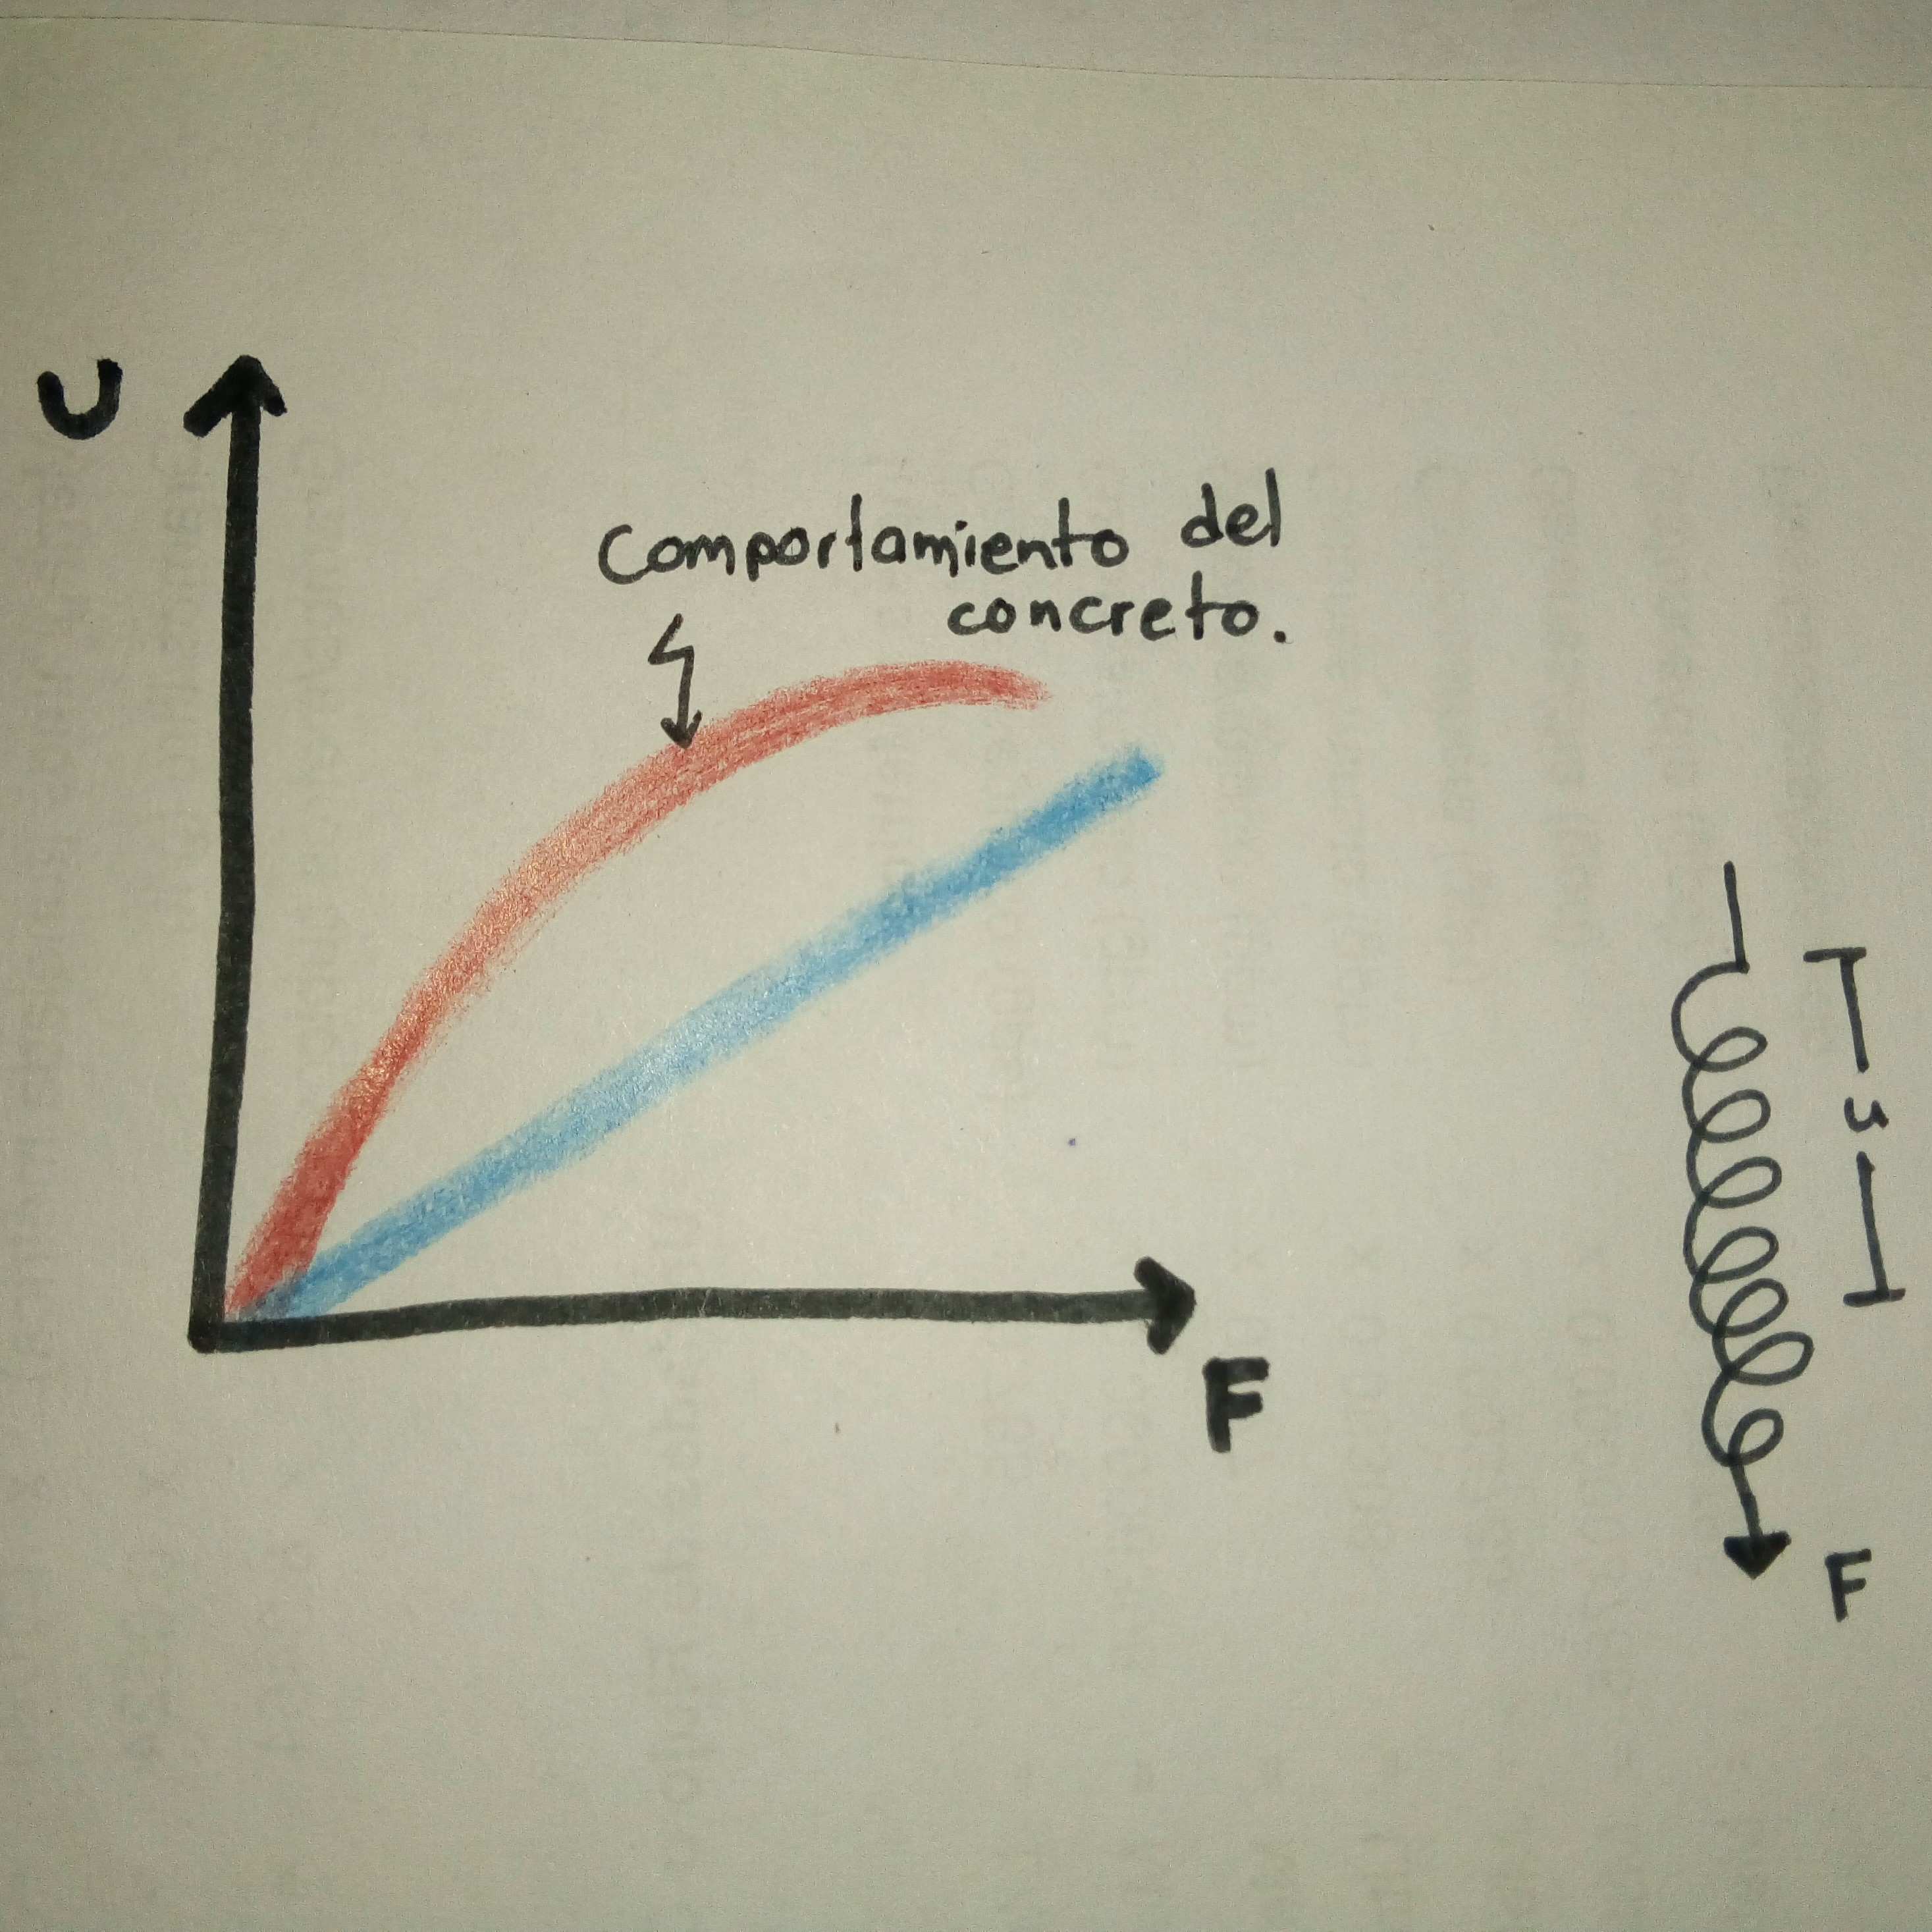
\includegraphics[scale=.05]{imagenes/13.jpg}
\end{center}
\end{center}
%ilustraciones de graficas y resorte%
$u=kF$\\
$u=k(u,F)$\\
\begin{displaymath}
f_1(x_1,x_2,x_3,x_4,\cdots, x_n)=0
\end{displaymath}
\begin{displaymath}
f_2(x_1,x_2,x_3,x_4,\cdots, x_n)=0
\end{displaymath}
\begin{displaymath}
f_3(x_1,x_2,x_3,x_4,\cdots, x_n)=0
\end{displaymath}
\begin{center}
$\vdots$
\end{center}
\begin{displaymath}
f_n(x_1,x_2,x_3,x_4,\cdots, x_n)=0
\end{displaymath}
\begin{displaymath}
F=\begin{bmatrix}
f_1(x)\\
f_2(x)\\
f_3(x)\\
\vdots \\
f_n(x)
\end{bmatrix}; \qquad x=\begin{bmatrix}
x_1\\
x_2\\
x_3\\
\vdots \\
x_n
\end{bmatrix}
\end{displaymath}
$F(x)=0; \qquad f(x)=0$\\
\begin{displaymath}
F(x^{k+1})=F(x^k)+F'(x^k)(x^{k+1}-x^k)\mid +F'(x^k)\frac{(x^{k+1}-x^k)^2}{2!}
\end{displaymath}
$0=F(x^k)+F'(x^k)(x^{k+1}-x^k)$\\
\begin{center}
Matriz Jacobiana del sistema
\end{center}
\begin{displaymath}
F'(x)=\begin{bmatrix}
\nabla f_1(x)^T \\
\nabla f_2(x)^T \\
\nabla f_3(x)^T \\
\vdots \\
\nabla f_n(x)^T
\end{bmatrix}=\begin{bmatrix}
\frac{\delta f_1}{\delta x_1} & \frac{\delta f_1}{\delta x_2} & \frac{\delta f_1}{\delta x_3} & \cdots & \frac{\delta f_1}{\delta x_n} \\
\frac{\delta f_2}{\delta x_1} & \frac{\delta f_2}{\delta x_2} & \frac{\delta f_2}{\delta x_3} & \cdots & \frac{\delta f_2}{\delta x_n} \\
\vdots & \vdots & \vdots & \ddots & \vdots \\ \frac{\delta f_n}{\delta x_1} & \frac{\delta f_n}{\delta x_2} & \frac{\delta f_n}{\delta x_3} & \cdots & \frac{\delta f_n}{\delta x_n} \\
\end{bmatrix}
\end{displaymath}
$s^k=x^{k+1}-x^k$\\
\begin{displaymath}
F'(x^k)(s^k)=-F(x^k)
\end{displaymath}
Se resuelve el sistema para obtener posteriormente el valor de $x^{k+1}$



%--------------------------------------%

\chapter{Derivadas num\'ericas parciales}
En el primer cap\'itulo hablamos de las derivadas num\'ericas, que hacen referencia a la derivaci\'on respecto a una sola varible. Habr\'a ocasiones en las que la soluc\'on de sistemas deber\'a ser dada por derivadas parciales, ya que los sistemas manejan m\'as de una variable, lo que hace necesario conocer acerca de esto.
%Algoritmo%
Dado $f(x,y)$
\begin{displaymath}
\frac{\delta f}{\delta x}=\lim_{\Delta x \to 0} \frac{f(x+\Delta x, y)-f(x,y)}{\Delta x}
\end{displaymath}
\begin{displaymath}
\frac{\delta f}{\delta y}=\lim_{\Delta y \to 0} \frac{f(x, y\Delta y)-f(x,y)}{\Delta y}
\end{displaymath}
\begin{displaymath}
\frac{\delta f}{\delta x}=\frac{f(x+h, y)-f(x,y)}{h} \qquad ; \qquad \frac{\delta f}{\delta y}=\frac{f(x, y+h)-f(x,y)}{h}
\end{displaymath}
\begin{displaymath}
\frac{\delta f}{\delta x_j}=\frac{f(x_1, x_2, \cdots , x_j+h, \cdots , x_n)-f(x_1,x_2,x_3, \cdots ,x_n)}{h}
\end{displaymath}
\begin{displaymath}
[F'(x)]_{ij}=\frac{f_j(x_1,x_2,x_j+h,\cdots ,x_n)-f_i(x_1, x_2, x_3,\cdots ,x_n)}{h}
\end{displaymath}
%--Hacer un ejemplo--%
\chapter{Calculo de Eigenvalores}
(Valores y vectores propios carecteristicos).
%--Intoducción al capítulo--%
%--Diagramas de resorte y tanque elevado--%
\begin{displaymath}
\frac{Md^2u}{dt^2}+c\frac{du}{dt}+kV=0
\end{displaymath}
\begin{displaymath}
\frac{Md^2u}{dt^2}+c\frac{du}{dt}+kV=f(t)
\end{displaymath}
\begin{displaymath}
\frac{Md^2u}{dt^2}+ku=0
\end{displaymath}
Donde $u=e^{at}$
\begin{displaymath}
\frac{du}{dt}=ae^{at} \qquad \frac{d^2V}{dt^2}=a^2e^{at}
\end{displaymath}
\begin{center}
$a^2Me^{at}+ke^{at}=0$\\
$a^2M+k=0$\\
$a^2M+k=0$
\end{center}
\begin{displaymath}
a=\sqrt{-\frac{k}{m}}=\sqrt{\frac{k}{m}}i
\end{displaymath}
\\
$Av=\lambda V$\\
$Av-\lambda V=0$\\
$(A-\lambda I)V=0\rightarrow$ Sistema lineal homogeneo tiene una soluci\'on trivial $v=0$
\\
\\
Para que $V\leq 0$
\begin{center}
$det(A-\lambda I)=0$\\ecuaci\'on polin\'omica de grado n.
\end{center} 

\begin{displaymath}
\begin{bmatrix}
a_{11} & a_{12} \\
a_{21} & a_{22}
\end{bmatrix}-\lambda \begin{bmatrix}
1 & 0 \\
0 & 1 
\end{bmatrix}
\end{displaymath}
\\
\begin{displaymath}
det\left| \begin{matrix}
a_{11}-\lambda & a_{12} \\
a_{21} & a_{22}-\lambda
\end{matrix}\right| =0
\end{displaymath}
\\
\begin{center}
$(a_{11}-\lambda)(a_{22}-\lambda)-a_{21}a_{12}=0$\\
$\lambda ^2-(a_{11}+a_{22})\lambda +a_{11}a_{22}-a_{11}a_{22}-a_{11}a_{12}=0$\\
\end{center}
\begin{displaymath}
\lambda =\frac{a_{11}+a_{22}\pm\sqrt{(a_{11}+a_{22})^2-4(a_{11}a_{22}-a_{21}a_{12})}}{2}
\end{displaymath}
\begin{displaymath}
-\frac{a_{21}}{a_{11}\lambda}\begin{bmatrix}
a_{11}-\lambda_1 & a_{12} \\
a_{21} & a_{22}\lambda_2
\end{bmatrix}\begin{bmatrix}
x\\y
\end{bmatrix}=\begin{bmatrix}
0 \\ 0
\end{bmatrix}
\end{displaymath}

\begin{displaymath}\begin{bmatrix}
a_{11}-\lambda_1 & a_{12} \\
0 & 0
\end{bmatrix}\begin{bmatrix}
x\\y
\end{bmatrix}=\begin{bmatrix}
0 \\ 0
\end{bmatrix}
\end{displaymath}
\begin{displaymath}
v_1=\begin{bmatrix}
-\frac{a_{12}y}{a_{11}-\lambda_1} \\
y
\end{bmatrix} \qquad v_2=\begin{bmatrix}
-\frac{a_{12}y}{a_{11}-\lambda_2} \\
y
\end{bmatrix}
\end{displaymath}
\subsection*{Propiedades}
\begin{itemize}
\item Los eigenvectores son linealmente independientes
\item Los igenvectores no son \'unicos, pero sus direcciones si lo son.
\item Si a es sim\'etrico, todos los eigenvectores son reales.
\item El rango de una matriz esta relacionado con el n\'umero de eigenvectores nulos
\end{itemize}
\section{M\'etodo de la potencia}
\subsection*{Hipotesis fundamental:}
Los eigenvalores de $A$, se pueden ordenar por valor absoluto en la forma
\begin{displaymath}
|\lambda_1|>|\lambda_2|\geq |\lambda_3|\geq|\lambda_4|\geq\cdots\geq|\lambda_n|
\end{displaymath}

Entonces empezando en un vector cualquiera $z_o\leq 0$ se tiene que la secuencia $z_{k+1}=Az_k$ converge a la direcci\'on $v_1$ si $k \to \infty$\\
\begin{displaymath}
Calcular \quad v_1=\frac{z_k}{\parallel z_k \parallel}
\end{displaymath}
\begin{center}
$v_1^TAv_1=r_1^T\lambda_1v_1$\\
$v_1^TAV_1=\lambda_1v_1^TV_1$\\
$\lambda_1=v_1^TAV_1$
\end{center}
Normalizar el vector resultante para obtener resultados aceptables y no haya problema de desbordamientp.
%---Algoritmo de potencia---%

\section{M\'etodo de iteraci\'on inversa}
Es un m\'etodo \'util cuando la matriz es simetrica y definida positiva.
\subsection*{Teorema}
Si $det(A)\leq 0,\quad A^{-1}$ existe y tiene los misos eigenvectors, corresponde a los de A por 
\begin{displaymath}
\frac{1}{\lambda_1},\frac{1}{\lambda_2},\frac{1}{\lambda_3},\cdots,\frac{1}{\lambda_n},
\end{displaymath}
%---Algoritmo de iteración inversa---%

\section{T\'ecnica de desplazamiento ("Shifting")}
Cuando se quieren encontrar los eigenvectores m\'as chiquitos, siempre y cuando la matriz sea definida positiva.\\
sirve para acelerar la convergencia, con el m\'etodo de la potencia trasladada.\\ 
$Av=\lambda v$\\
La matriz $A+\theta I$ tiene los mismos eigenvectores que $A$, y sus eigenvectores son $\theta +\lambda$.
$(A+\theta I)v=Av+\theta Iv=Av+\theta v$
\\
$(A+\theta I)v=Av+\theta Iv=\lambda v+\theta v$\\
$(A+\theta I)v=(\lambda+\theta)v=(\lambda+\theta)v$
\section{T\'ecnicas de deflaci\'on}
Se obtiene una nueva matriz $B$ de manera que contenga los mismos eigenvectores de $A$, pero uno de sus eigenvectores se reemplaza por uncero.
\begin{center}
$Bv=\lambda 'v$\\
$Av=\lambda v$
\end{center}
Si $A$ es sim\'etrica, $B$ se obtiene por $B=A-\lambda_1v_1v_1^T$
 
\section{M\'etodo del polinomio}
se puede aplicar la t\'ecnica de desplazamiento.
\begin{displaymath}
det(A-I\lambda)=0
\end{displaymath} 
\begin{center}
$f(\lambda)=0$\\
$f(x)=0$\\
$LU=A$\\
$det(A)=det(L)det(U)$
\end{center}
\chapter{Interpolaci\'on}
\chapter{Integraci\'on num\'erica}

\end{document}